\documentclass[xetex,mathserif,serif]{beamer}

\setbeamertemplate{caption}[numbered]
% Hyperlinks.
\usepackage{hyperref}

% Language settings.
\usepackage{polyglossia}
\setdefaultlanguage[babelshorthands=true]{russian}

% Setting outer theme.
\useoutertheme{infolines}

% Setting font.
\usepackage{fontspec}
\setmainfont{FreeSans}
\newfontfamily{\russianfonttt}{FreeSans}

% Code highlighting.
\usepackage[outputdir=build]{minted}
\usepackage{xcolor}

% Images.
\usepackage{graphicx}
\usepackage{animate}
\usepackage{subfig}


\usepackage{mathtools}

\title[СПбГУ]{Построение гибридной рекомендательной
системы новостей с применением методов
оптимизации}
\author[Смирнов Александр 17.Б07-мм]{Смирнов Александр 17.Б07-мм}
\institute[]{Научный руководитель: к.ф.-м.н., доц. Михайлова Елена Георгиевна \\
             Рецензент: руководитель отдела инженерии ООО ``АЙ ТИ Сервис'', Осипов Евгений Валерьевич}
% \author[Alexander Smirnov]{Alexander Smirnov\\ \footnotesize supervisor: Elena Mikhailova}

\begin{document}


\frame{\titlepage}

% \section{Introduction}

% \subsection{Approaches}

\begin{frame}
	\frametitle{Введение}

	\begin{itemize}
		\item Приложение ЯRUS:
		      \begin{itemize}
			      \item Агрегатор новостей;
			      \item Социальная сеть;
		      \end{itemize}
		\item Огромный объём информации:
		      \begin{itemize}
			      \item Необходима персонализация.
		      \end{itemize}
	\end{itemize}

\end{frame}



\begin{frame}
	\frametitle{Постановка задачи}

	\begin{itemize}
		\item Цель:
            \begin{itemize}
                \item Реализация рекомендательной системы новостей в приложении ЯRUS;
            \end{itemize}

		\item Задачи:
            \begin{itemize}
                \item Исследование предметной области;
                \item Анализ проблем существующих подходов;
                \item Реализация подходов;
                \item Совмещение подходов в единую систему;
                \item Анализ качества работы рекомендательной системы;
                \item Оценка влияния решения на ключевые показатели эффективности.
            \end{itemize}
	\end{itemize}
\end{frame}


\begin{frame}
	\frametitle{Проблемы}

	\begin{itemize}
		\item Проблемы:
		      \begin{itemize}
			      \item Холодный старт;
			      \item Вычислительные затраты
			      \item Разреженность данных
			      \item 
		      \end{itemize}
		\item clickbait
		\item 
	\end{itemize}
\end{frame}


\begin{frame}
	\frametitle{Описание модели}

	\begin{itemize}
		\item веса меняются со временем работы алгоритма
		\item геолокация
		\item 
	\end{itemize}
\end{frame}

\begin{frame}
	\frametitle{Content-based approach}

	\begin{figure}[h]
		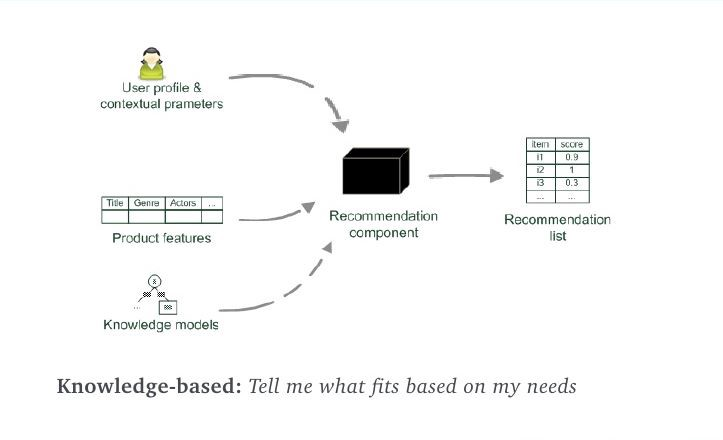
\includegraphics[width=0.9\textwidth]{./images/content_based.jpeg}
		\centering
	\end{figure}
\end{frame}


\begin{frame}
	\frametitle{Collaborative approach}

	\begin{figure}[h]
		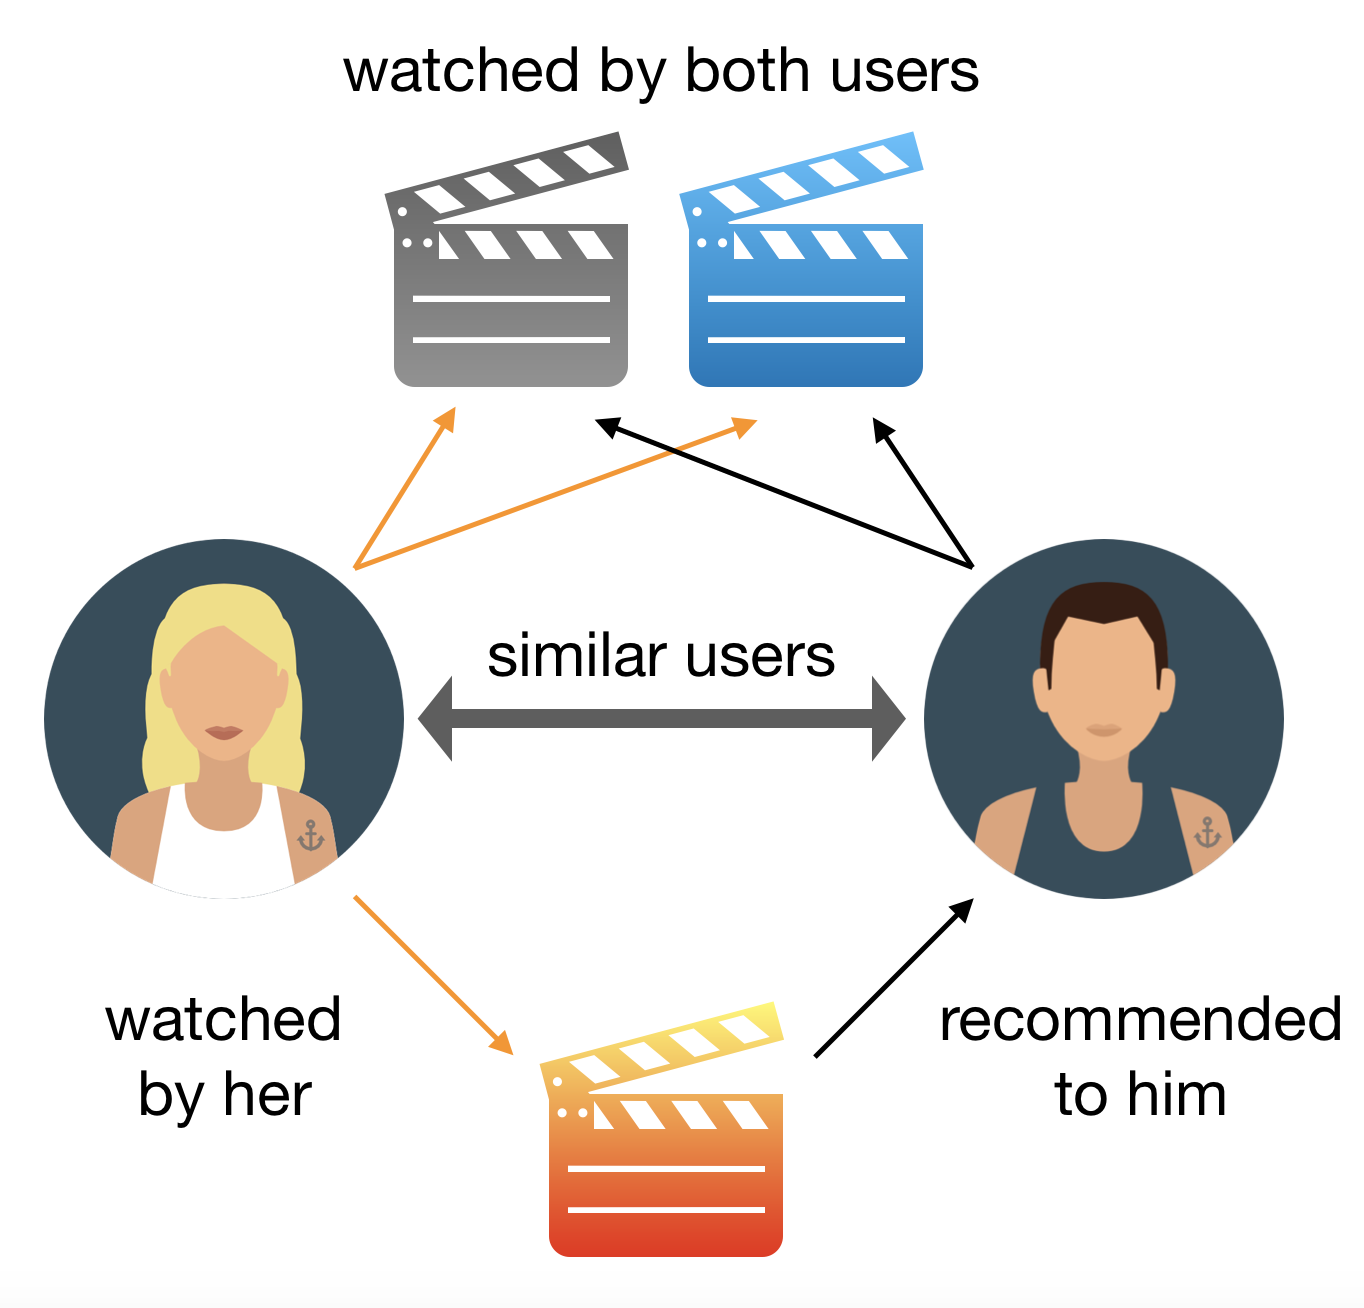
\includegraphics[width=0.5\textwidth]{./images/collaborative.png}
		\centering
	\end{figure}
\end{frame}



\begin{frame}
	\frametitle{Goal}

	\begin{itemize}
		\item Scalable hybrid news recommender system
		\item Use as many information as possible
		      \begin{itemize}
			      \item users' logs
			            \begin{itemize}
				            \item likes
				            \item comments
				            \item views
				            \item shows
				            \item etc
			            \end{itemize}
			      \item news' features
			            \begin{itemize}
				            \item source
				            \item popularity
				            \item theme
				            \item etc
			            \end{itemize}
		      \end{itemize}
	\end{itemize}
\end{frame}


\begin{frame}
	\frametitle{Solution}

	\begin{itemize}
		\item Hybrid recommender
		      \begin{itemize}
			      \item Collaborative recommender
			      \item Content-based recommender
			      \item Last Viewed recommender
			      \item Boost recommender
		      \end{itemize}
		\item Optimize weights
	\end{itemize}
\end{frame}

\begin{frame}
    \frametitle{Оценка качества (offline)}

	\begin{itemize}
		\item MAP@20
		\item NDCG
		\item 
	\end{itemize}
\end{frame}


\begin{frame}
	\frametitle{Оценка качества (online)}

	\begin{itemize}
		\item A/B тестирование:
            \begin{itemize}
                \item Время нахождения на вкладке ``новости'' за одну сессию;
            \end{itemize}
		\item 
		\item 
	\end{itemize}
\end{frame}

\begin{frame}
	\frametitle{Апробация}

    \begin{figure}[h]
        
\includegraphics[width=0.3\textwidth]{./images/screenshot.png}
        \caption{Персонализированная рекомендательная лента}
        \label{fig:feed}
        \centering
    \end{figure}

\end{frame}


\begin{frame}
	\frametitle{Результаты}
	\begin{itemize}
		\item 
		\item 
		\item 
	\end{itemize}
\end{frame}


\begin{frame}
	\frametitle{Акт о внедрении}

    \begin{figure}[h]
        
\includegraphics[width=0.45\textwidth]{./images/akt.jpg}
        \caption{Акт о внедрении}
        \label{fig:akt}
        \centering
    \end{figure}

\end{frame}

\end{document}
